\subsection{Hydrogen production methods}
\begin{frame}
\frametitle{Electrolysis}
\begin{columns}
    \column[t]{5cm}
	\begin{figure}[htbp!]
		\begin{center}
			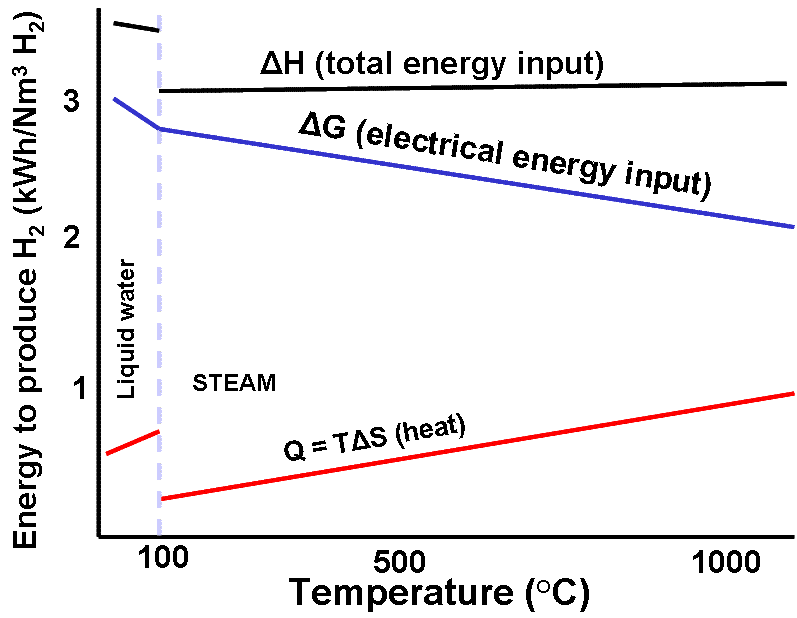
\includegraphics[height=4.0cm]{images/ele-curve.png}
		\end{center}
		\caption{Energy consumption of an ideal electrolysis process. Image reproduced from \cite{hi2h2_highly_2007}.}
	\end{figure}

	\column[t]{5cm}
	$\Delta H = \Delta G + T \Delta S$
	\begin{itemize}
		\item $\Delta$G: Electrical energy.
		\item T$\Delta$S: Thermal energy.
	\end{itemize}
    \vspace{0.7cm}

	\begin{itemize}
    	\item In low temperature electrolysis (LTE), electricity provides the thermal energy.
    	\item In high temperature electrolysis (HTE), a heat source provides the thermal energy.
    	\item HTE has the advantage of decreasing the electricity requirement.
    \end{itemize}
\end{columns}
\end{frame}


\begin{frame}
\frametitle{Sulfur-Iodine}
\begin{columns}
    \column[t]{5cm}
   	\begin{figure}[htbp!]
		\begin{center}
			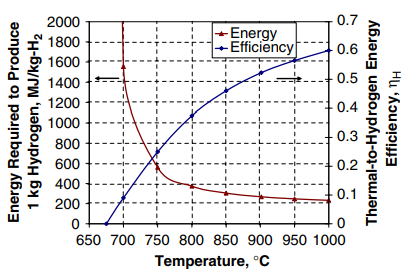
\includegraphics[height=4.0cm]{images/si-energy.png}
		\end{center}
		\caption{Sulfur-Iodine thermochemical cycle. Image reproduced from \cite{nomura_mikihiro_efficient_2004}.}
 	\end{figure}

 	\column[t]{5cm}
 	\begin{itemize}
 		\item 3 different reactions: sulfuric acid decomposition, Bunsen reaction, and hydrogen iodide decomposition.
 		\item Input: H$_2$O.
 		\item Output: H$_2$ $\&$ O$_2$. 
 		\item Does not require electricity.
 		\item Needs a high temperature source.
 	\end{itemize}
\end{columns}
\end{frame}


\subsection{Nuclear energy-based hydrogen}
\begin{frame}
\frametitle{Co-generation}
\begin{columns}
    \column[t]{6.8cm}
   	\begin{figure}[htbp!]
		\begin{center}
			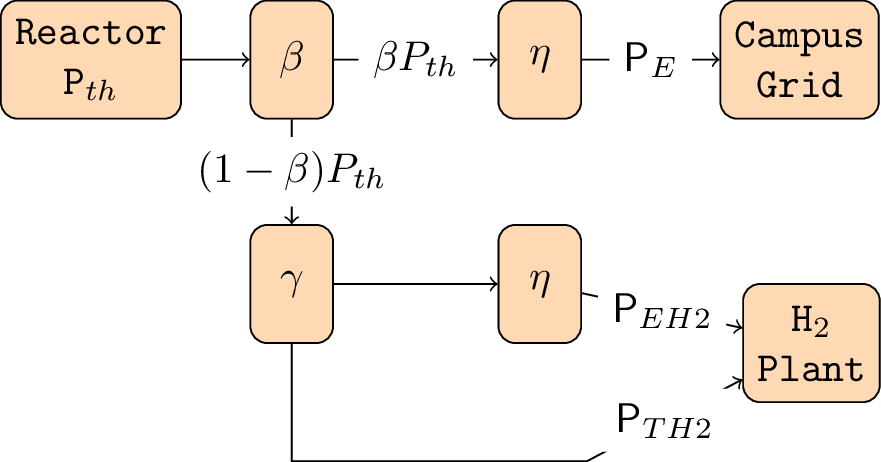
\includegraphics[height=3.6cm]{images/hte-figure0.png}
		\end{center}
		\caption{Diagram of a reactor coupled to hydrogen plant.}
 	\end{figure}

 	\column[t]{4.5cm}
 	$\beta$: power fraction that is converted into electricity.
 	\\
    $\beta$ = 1: no hydrogen produced.
    \\
 	$\beta$ = 0: no electricity produced. \vspace{0.5cm}

 	Low temperature electrolysis (LTE):
 	\begin{itemize}
 		\item $\gamma$=1. P$_{TH2}$ = 0.
 	\end{itemize}

 	High temperature electrolysis (HTE):
 	\begin{itemize}
 		\item 0 $< \gamma <$ 1.
 	\end{itemize}

    Sulfur-Iodine (SI):
 	\begin{itemize}
 		\item $\gamma$=0. P$_{EH2}$ = 0.
 	\end{itemize}
\end{columns}
\end{frame}